Esta seção apresenta a análise de dados de uso de processador e memória RAM da máquina virtual para a execução dos experimentos.
Os dados para cada contêiner foram agrupados em três conjuntos, para facilitar a visualização dos dados.
O primeiro conjunto representa os dados agregados de todas as instâncias do testador, denominado nos gráficos como Testadores.
O segundo conjunto representa os dados agregados de todas as funções do núcleo em teste, denominado nos gráficos como Núcleo.
O terceiro conjunto representa os dados agregados do restante dos serviços em execução, como os contêineres utilizados para rodar o módulo de coleta de dados do núcleo e o servidor da aplicação \textit{iPerf} utilizada no segundo experimento, denominado nos gráficos como Outros.
Uma análise com maiores detalhes do uso de recursos para cada componente em execução durante o período do experimento é possível ao utilizar a ferramenta para gerar visualizações dos dados coletados disponível através da aplicação \textit{InfluxDB}.
Essa ferramenta faz parte do módulo de coleta de dados do núcleo da rede.

\subsection{Análise e discussão em relação ao consumo de recursos do experimento de registro e estabelecimento de sessão do núcleo 5G}

Para a análise do uso de recursos de processador e memória RAM para a execução do experimento de registro e estabelecimento de sessão do núcleo 5G, foi utilizada uma execução do experimento com intervalo entre conexões de UEs de 500 ms sobre a máquina virtual com 12 núcleos de processador virtuais e 8 GB de memória RAM.
Os resultados agregados podem ser vistos na Figura \ref{fig:exp1_500ms_res}.

\begin{figure}[H]
    \centering
    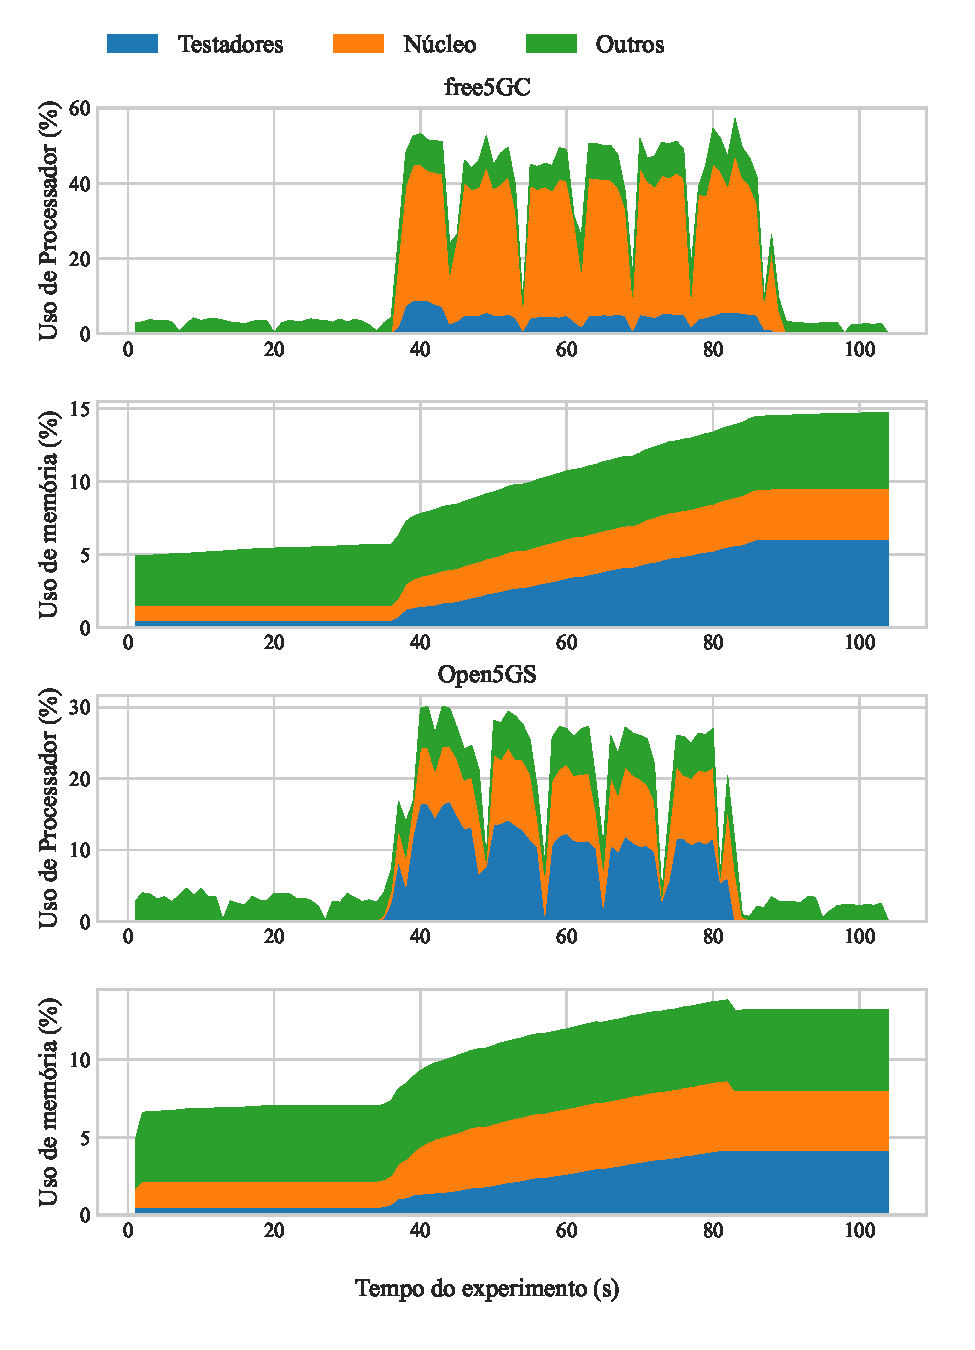
\includegraphics[width=0.95\textwidth]{TG2/Chapters/DataAnalysis/Figures/EXP1-CONN-RES-500ms-12C-8GB.pdf}
    \caption{Uso de processador e memória RAM para a execução com atraso de 500 ms entre conexões}
    \label{fig:exp1_500ms_res}
\end{figure}

Esta figura apresenta o uso de processador e memória RAM de acordo com o tempo de execução do experimento para os núcleos \textit{free5GC} e \textit{Open5GS}.
O eixo X dos gráficos representam o tempo em segundos referente à coleta de dados total do experimento, considerando o tempo para a inicialização, execução e encerramento do experimento.
O eixo Y representa a porcentagem do uso para cada tipo de recurso analisado.
As áreas azuis, laranjas e verdes dos gráficos representam a porcentagem de uso agregado de recursos para a execução dos testadores, núcleos 5G e os demais componentes, respectivamente.

Ao observar o uso de recursos somente durante o período da execução do experimento, a média de uso de processador para o núcleo \textit{free5GC} foi de 31,33\% e para o núcleo \textit{Open5GS} foi de 7,26\%.
Em relação ao uso de memória RAM, o pico de uso de memória para o núcleo \textit{free5GC} foi de 3.45\%, representando o uso de 282,6 MB de memória RAM.
Quanto ao núcleo \textit{Open5GS}, o pico de uso de memória RAM foi de 4,47\%, representando o uso de 366,2 MB de memória RAM.
Os resultados descritos acima demonstram que o núcleo de rede 5G \textit{Open5GS} apresentou uma performance 4.3x superior em relação ao uso de processador em comparação com o núcleo \textit{free5GC}.
Entretanto, em relação ao uso de memória RAM, o núcleo \textit{free5GC} apresentou uma performance 1.29x superior ao núcleo \textit{Open5GS}.


\subsection{Análise e discussão em relação ao consumo de recursos do experimento de desempenho do plano de dados}

Para realizar a análise do uso de recursos durante a execução do experimento para a avaliação do desempenho do plano de dados, foi escolhida as métricas de uso de recursos do processador e memória RAM.
Essa análise complementa a explicação do experimento demonstrada na Seção \ref{sec:results-dataplane-analysis}.
Os experimentos foram conduzidos em quatro configurações diferentes.
Entretanto, a análise do consumo de recursos foi focada em apenas duas configurações, com a maior e com a menor quantidade de recursos.
Ao observar os resultados do plano de dados para a execução do experimento de desempenho do plano de dados na máquina virtual com 12 núcleos virtuais e 8 GB de memória RAM, percebe-se que o desempenho máximo para o plano de dados do núcleo \textit{free5GC} com essa configuração de máquina virtual não foi atingido.
Esse resultado pode ser visto nos gráficos da Figura \ref{fig:exp2_10gnb_12c}.


\begin{figure}[H]
    \centering
    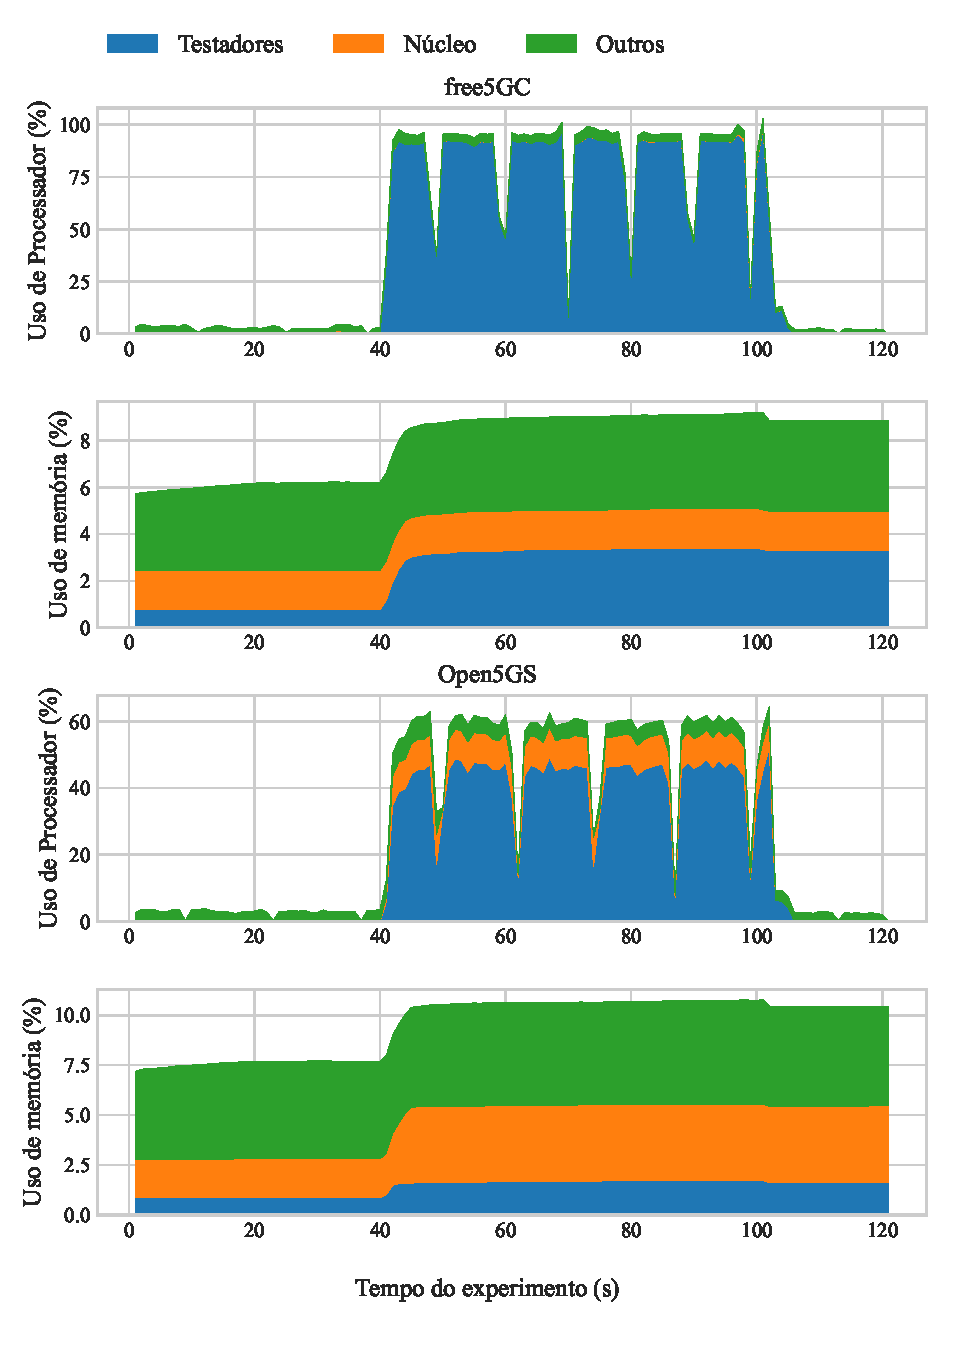
\includegraphics[width=0.95\textwidth]{TG2/Chapters/DataAnalysis/Figures/EXP2-IPERF-RES-10gNB-12C-8GB.pdf}
    \caption{Uso de processador e memória RAM para o experimento de desempenho de plano de dados com 10 UEs conectados}
    \label{fig:exp2_10gnb_12c}
\end{figure}

É possível observar que o uso médio de processador durante a execução desse experimento foi de 95,57\% para o núcleo \textit{free5GC}, com poucos picos de uso atingindo os 100\%.
Do total de uso de processador, 91,87\% do uso é representado pelos testadores e UEs realizando os testes.
O uso de processador médio do núcleo \textit{free5GC} durante a execução do experimento foi de 0,03\%.
Isso demonstra que o núcleo de rede 5G utiliza poucos recursos de processador para realizar o gerenciamento do plano de dados dos UEs conectados.

Em relação ao núcleo \textit{Open5GS}, que não é otimizado para o gerenciamento do plano de dados de múltiplos UEs em paralelo, o uso de processador médio total durante a execução do experimento foi de 59,59\%.
O total de uso de processador durante a execução de experimento é dividida principalmente entre as instâncias do testador e o núcleo da rede 5G, com o testador representando 45,95\% do uso do processador e o núcleo representando 8,96\%.
A redução de uso de processador pelas instâncias do testador e UEs em relação ao experimento executado com o núcleo \textit{free5GC} é explicada pela baixa largura de banda disponível pelo \textit{Open5GS}.

Uma possível explicação desses resultados é que o núcleo \textit{free5GC} provavelmente utiliza paralelização para gerenciar o processamento do plano de dados dos UEs.
Isso provavelmente justificaria a facilidade em escalar a quantidade de UEs conectados reduzindo sutilmente o desempenho individual dos UEs.
Por outro lado, o núcleo \textit{Open5GS} não apresenta o mesmo comportamento.
De acordo com os resultados, o núcleo utilizou 8,96\% do total de processamento disponível na máquina virtual.
Isso é equivalente a um pouco mais que a capacidade de um núcleo do processador disponível.
Possivelmente, este núcleo não está otimizado para paralelizar o processamento do plano de dados quando múltiplos UEs estão conectados.
Isso explicaria o baixo desempenho observado nos resultados do núcleo \textit{Open5GS}.

Ao observar o uso de recursos de processador para a máquina virtual com 4 núcleos virtuais de processador e 4 GB de memória RAM, é possível explicar a queda de desempenho para o plano de dados do núcleo \textit{free5GC} após os testes com mais de 4 UEs simultâneos.
A Figura \ref{fig:exp2_4gnb_4c} representa os gráficos de uso de processador e memória RAM para uma execução do experimento de desempenho do plano de dados 

\begin{figure}[H]
    \centering
    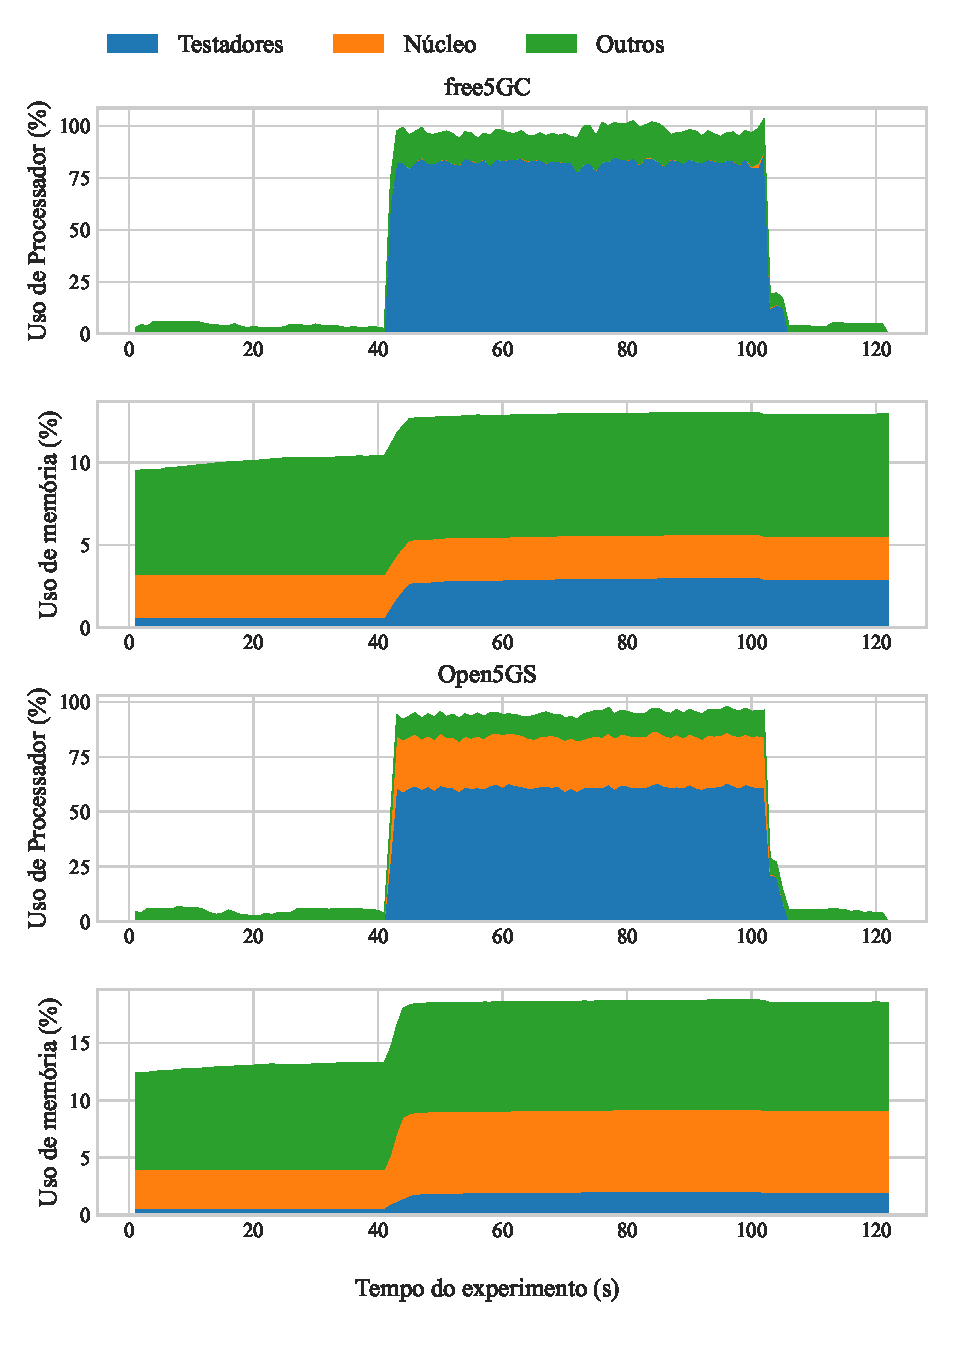
\includegraphics[width=0.95\textwidth]{TG2/Chapters/DataAnalysis/Figures/EXP2-IPERF-RES-4gNB-4C-4GB.pdf}
    \caption{Uso de processador e memória RAM para o experimento de desempenho de plano de dados com 4 UEs conectados}
    \label{fig:exp2_4gnb_4c}
\end{figure}

É possível observar que o uso do processador para a execução de quatro UEs conectados e utilizando o plano de dados do núcleo de rede 5G \textit{free5GC} está muito próximo de 100\%, atingindo o uso máximo do processador em diversos momentos.
Dessa forma, é possível perceber que o máximo de UEs simultâneos que essa configuração de máquina virtual suporta são quatro.
Para quantidades superiores a quatro UEs simultâneos, a redução de desempenho do plano de dados é explicada devido ao chaveamento necessário realizado pelo sistema operacional para gerenciar os diversos processos executando em paralelo.
